\documentclass[submit]{harvardml}

% FDV: Check all frontmatter for years, due dates, and references for
% sections of the textbook, etc.
\course{CS181-S22}
\assignment{Assignment \#3}
\duedate{11:59pm EST, March 11, 2022}

\usepackage[OT1]{fontenc}
\usepackage[colorlinks,citecolor=blue,urlcolor=blue]{hyperref}
\usepackage[pdftex]{graphicx}
\usepackage{subfig}
\usepackage{fullpage}
\usepackage{amsmath}
\usepackage{amssymb}
\usepackage{color}
\usepackage{soul}
\usepackage{todonotes}
\usepackage{listings}
\usepackage{common}
\usepackage{enumitem}
\usepackage{bm}
\newcommand{\B}{\text{B}}
\newcommand{\Beta}{\text{Beta}}
\usepackage{pythonhighlight}
\usepackage[mmddyyyy,hhmmss]{datetime}

\usepackage{comment}
\newcommand{\TODO}{{\color{red}TODO }}

\setlength\parindent{0em}

\definecolor{verbgray}{gray}{0.9}

\lstnewenvironment{csv}{%
  \lstset{backgroundcolor=\color{verbgray},
  frame=single,
  framerule=0pt,
  basicstyle=\ttfamily,
  columns=fullflexible}}{}

\begin{document}

\begin{center}
{\Large Homework 3: Bayesian Methods and Neural Networks}\\
\end{center}

% FDV: Update for resources, accuracy of submit information **especially any colab components**
% FDV: Make sure to emphasize any plots must be in the pdf submission, we will not be checking code / source 
\subsection*{Introduction}

This homework is about Bayesian methods and Neural Networks.  Section 2.9 in the textbook as well as reviewing MLE and MAP will be useful for Q1. Chapter 4 in the textbook will be useful for Q2.

Please type your solutions after the corresponding problems using this
\LaTeX\ template, and start each problem on a new page.

Please submit the \textbf{writeup PDF to the Gradescope assignment `HW3'}. Remember to assign pages for each question.  \textbf{All plots you submit must be included in your writeup PDF.  }We will not be checking your code / source files except in special circumstances. 

Please submit your \textbf{\LaTeX file and code files to the Gradescope assignment `HW3 - Supplemental'}. 

% FDV: Last year, we pointed folks to
% https://www.cs.ubc.ca/~murphyk/Papers/bayesGauss.pdf
% and folks ended up basically copying from it and not doing any derivation
% For this year, I modified to ask folks to do the full derivation in
% 1.1 but then give them the formula for the marginal likelihood so
% they don't have to derive that.  Open to other variations:
% basically, I think it's probably okay for one part to have a longer
% derivation, but if folks think it's too much, we could have students
% refer to the paper above again or just give them the formula for 1.1
% and ask them to simply interpret it.

\newpage


\begin{problem}[Bayesian Methods]

  This question helps to build your understanding of making
  predictions with a maximum-likelihood estimation (MLE), a maximum a
  posterior estimator (MAP), and a full posterior predictive.

  Consider a one-dimensional random variable $x = \mu + \epsilon$,
  where it is known that $\epsilon \sim N(0,\sigma^2)$.  Suppose we
  have a prior $\mu \sim N(0,\tau^2)$ on the mean. You observe iid data $\{x_i\}_{i=1}^n$ (denote the data as $D$).


\textbf{We derive the distribution of $x|D$ for you.}

\textbf{The full posterior predictive is computed using:}

$$p(x|D)=\int p(x, \mu|D) d\mu =\int p(x|\mu)p(\mu|D) d\mu $$


\textbf{One can show that, in this case, the full posterior predictive distribution has a nice analytic
  form:}
   \begin{align}
        x|D \sim \mathcal{N}\Bigg(\frac{\sum_{x_i\in D}x_i}{n+\frac{\sigma^2}{\tau^2}}, (\frac{n}{\sigma^2}+\frac{1}{\tau^2})^{-1} + \sigma^2\Bigg)
     \end{align}

\begin{enumerate}

  \item Derive the distribution of $\mu|D$.

  \item 
  In many problems, it is often difficult to
  calculate the full posterior because we need to marginalize out the parameters as above (here,
  the parameter is $\mu$). We can mitigate this problem by plugging in
  a point estimate of $\mu^*$ rather than a distribution.

  a) Derive the MLE
  estimate $\mu_{MLE}$.
  % using $p(D|\mu)$.
  
  b) Derive the MAP estimate $\mu_{MAP}$. % using $p(\mu|D)$

  c) What is the relation between $\mu_{MAP}$ and the mean of $x|D$?

  d) For a fixed value of $\mu=\mu^*$, what is the distribution of $x|\mu^*$? Thus, what is the distribution of $x|\mu_{MLE}$ and $x|\mu_{MAP}$?

  e) Is the variance of $x|D$ greater or smaller than the variance of $x|\mu_{MLE}$? What is the limit of the variance of $x|D$ as $n$ tends to infinity? Explain why this is intuitive.


\item Let us compare $\mu_{MLE}$  and $\mu_{MAP}$. There are three cases to consider:

 a) Assume $\sum_{x_i \in D} x_i=0$. What are the values of $\mu_{MLE}$ and $\mu_{MAP}$?

 b) Assume $\sum_{x_i \in D} x_i>0$. Is $\mu_{MLE}$ greater than $\mu_{MAP}$?

 c) Assume $\sum_{x_i \in D} x_i<0$. Is $\mu_{MLE}$ greater than $\mu_{MAP}$?
  
    
\item Compute:

$$\lim_{n \rightarrow \infty} \frac{\mu_{MAP}}{\mu_{MLE}}$$

  \end{enumerate}

  \end{problem}

\subsection*{Solution:}

\begin{enumerate}
	\item By Bayes' rule,
	$$p(\mu|D) = \frac{p(D|\mu)p(\mu)}{p(D)} \propto p(D|\mu)p(\mu).$$
	We will drop various terms throughout the derivation that are constant with respect to $\mu$, as the final distribution for $\mu|D$ will be renormalized to integrate to unity. Using the definition of the Gaussian PDF, the likelihood of the data is
	$$p(D|\mu) = \prod_{i=1}^n \mathcal{N}(x_i | \mu, \sigma^2) = \prod_{i=1}^n \frac{1}{\sigma \sqrt{2\pi}} \exp\left\{-\frac12\frac{(x_i - \mu)^2}{\sigma^2}\right\} \propto \exp\left\{-\frac12\frac{\sum_{i=1}^n(x_i - \mu)^2}{\sigma^2}\right\}$$
	and the prior on $\mu$ is
	$$p(\mu) = \mathcal{N}(\mu | 0, \tau^2) = \frac{1}{\tau \sqrt{2\pi}} \exp\left\{-\frac12\frac{(\mu - 0)^2}{\tau^2}\right\} \propto \exp\left\{-\frac12\frac{\mu^2}{\tau^2}\right\}.$$
	Therefore,
	$$p(\mu | D) \propto \exp\left\{-\frac12\left(\frac{\sum_{i=1}^n(x_i - \mu)^2}{\sigma^2} + \frac{\mu^2}{\tau^2}\right)\right\}.$$
	The product of two Gaussian PDFs is Gaussian, so we want to re-arrange the above expression to be proportional to a new Gaussian PDF with parameters $\mu_n$ and $\sigma_n$,
	$$\mathcal{N}(\mu | \mu_n, \sigma_n) \propto \exp\left\{-\frac12 \frac{(\mu - \mu_n)^2}{\sigma_n^2}\right\} = \exp\left\{-\frac12 \left(\mu^2\frac{1}{\sigma_n^2} -2 \mu\frac{\mu_n}{\sigma_n^2} + \frac{\mu_n^2}{\sigma_n^2}\right)\right\}.$$
	Expanding the squared term in our expression for $p(\mu|D)$ and rearranging,
	\begin{align*}
		p(\mu | D) &\propto \exp\left\{-\frac12\left(\frac{\sum_{i=1}^n x_i^2}{\sigma^2} -2\mu \frac{\sum_{i=1}^n x_i}{\sigma^2} + \frac{n\mu^2}{\sigma^2} + \frac{\mu^2}{\tau^2}\right)\right\} \\
		&= \exp\left\{-\frac12\left(\mu^2\left(\frac{1}{\tau^2} + \frac{n}{\sigma^2}\right) -2\mu\frac{\sum_{i=1}^n x_i}{\sigma^2} + \frac{\sum_{i=1}^n x_i^2}{\sigma^2} \right)\right\}.
	\end{align*}
	Matching up terms in the expression above with the Gaussian PDF expression we want,
	$$\mu^2\left(\frac{1}{\tau^2} + \frac{n}{\sigma^2}\right) = \mu^2 \frac{1}{\sigma_n^2} \Rightarrow \sigma_n^2 = \left(\frac{1}{\tau^2} + \frac{n}{\sigma^2}\right)^{-1}$$
	and
	$$-2\mu\frac{\sum_{i=1}^n x_i}{\sigma^2} = -2\sigma\frac{\mu_n}{\sigma_n^2} \Rightarrow \mu_n = \left(\frac{1}{\tau^2} + \frac{n}{\sigma^2}\right)^{-1} \frac{\sum_{i=1}^n x_i}{\sigma^2}.$$
	Therefore,
	$$\mu | D \sim \mathcal{N}(\mu_n, \sigma_n^2) = \mathcal{N}\left(\left(\frac{1}{\tau^2} + \frac{n}{\sigma^2}\right)^{-1} \frac{\sum_{i=1}^n x_i}{\sigma^2}, \left(\frac{1}{\tau^2} + \frac{n}{\sigma^2}\right)^{-1}\right).$$
	
	\item 
	\begin{enumerate}
	
		\item To find $\mu_{MLE} \in \arg \max_\mu p(D|\mu)$, take the logarithm of the likelihood, differentiate, and set equal to zero:
		\begin{align*}
			p(D|\mu) &= \prod_{i=1}^n p(x_i | \mu)
			= \prod_{i=1}^n \mathcal{N}(x_i | \mu, \sigma^2) \\
			&= \prod_{i=1}^n \frac{1}{\sigma\sqrt{2\pi}}\exp\left\{-\frac12 \frac{(x_i - \mu)^2}{\sigma^2}\right\} \\
			&= \frac{1}{\sigma\sqrt{2\pi}} \exp\left\{-\frac12 \frac{\sum_{i=1}^n (x_i - \mu)^2}{\sigma^2}\right\} \\
			\log p(D|\mu) &= \frac{1}{\sigma\sqrt{2\pi}} - \frac12 \frac{\sum_{i=1}^n (x_i - \mu)^2}{\sigma^2} \\
			\frac{\partial \log p(D|\mu)}{\partial \mu} &= \frac{1}{\sigma^2} \sum_{i=1}^n(x_i - \mu) \\
			0 &= \frac{1}{\sigma^2} \sum_{i=1}^n(x_i - \mu_{MLE}) \\
			\mu_{MLE} &= \frac{\sum_{i=1}^n x_i}{n},
		\end{align*}
		so $\mu_{MLE}$ is the empirical mean.
			
		\item To find $\mu_{MAP} \in \arg \max_\mu p(\mu|D)$, use the PDF of the Gaussian distribution derived in part (1), take the logarithm, differentiate, and set equal to zero:
		\begin{align*}
			p(\mu|D) &= \mathcal{N}(\mu | \mu_n, \sigma_n^2)
			= \frac{1}{\sigma_n\sqrt{2\pi}} \exp\left\{-\frac12 \frac{(\mu - \mu_n)^2}{\sigma_n^2}\right\} \\
			\log p(\mu|D)&= \log \left(\frac{1}{\sigma_n\sqrt{2\pi}}\right) -\frac12 \frac{(\mu - \mu_n)^2}{\sigma_n^2} \\
			\frac{\partial \log p(\mu|D)}{\partial \mu} & = -\frac{\mu - \mu_n}{\sigma_n^2} \\
			0 &= -\frac{\mu_{MAP} - \mu_n}{\sigma_n^2} \\
			\mu_{MAP}&= \mu_n = \left(\frac{1}{\tau^2} + \frac{n}{\sigma^2}\right)^{-1} \frac{\sum_{i=1}^n x_i}{\sigma^2}.
		\end{align*}
		In this case, we could also have seen that $\mu_{MAP} = \mu_n$ by recognizing that the most likely value of $\mu|D$ is the mean of its distribution.
	
	\item We have
	$$\mu_{MAP} = \left(\frac{1}{\tau^2} + \frac{n}{\sigma^2}\right)^{-1} \frac{\sum_{i=1}^n x_i}{\sigma^2} = \frac{\sum_{i = 1}^n x_i}{\left(\frac{1}{\tau^2} + \frac{n}{\sigma^2}\right) \sigma^2} = \frac{\sum_{x_i \in D} x_i}{n + \frac{\sigma^2}{\tau^2}},$$
	so $\mu_{MAP}$ is equal to the mean of $x|D$.
	
	\item For a fixed value of $\mu = \mu^*$, the distribution of $x|\mu^*$ is $\mathcal{N}(\mu^*, \sigma^2)$, since $x \sim \mu^* + \epsilon \sim \mathcal{N}(\mu^* + 0, 0 + \sigma^2)$. Thus,
	$$x|\mu_{MLE} \sim \mathcal{N}\left(\frac{\sum_{x_i \in D} x_i}{n}, \sigma^2\right)$$
	$$x|\mu_{MAP} \sim \mathcal{N}\left(\frac{\sum_{x_i \in D} x_i}{n + \frac{\sigma^2}{\tau^2}}, \sigma^2\right).$$
	
	\item The variance of $x|D$ is $\left(\frac{n}{\sigma^2} + \frac1{\tau^2}\right)^{-1} + \sigma^2$, which is greater than $\sigma^2$, the variance of $x|\mu_{MLE}$, because
	$$\left(\frac{n}{\sigma^2} + \frac1{\tau^2}\right)^{-1} > 0,$$
	for all $n>0$, assuming $\sigma^2, \tau^2 > 0$. The limit of the variance of $x|D$ as $n$ tends to infinity is
	$$\lim_{n \rightarrow \infty} \left(\left(\frac{n}{\sigma^2} + \frac1{\tau^2}\right)^{-1} + \sigma^2\right) = \lim_{n \rightarrow \infty} \left(\left(\frac{n}{\sigma^2} + \frac1{\tau^2}\right)^{-1}\right) + \sigma^2 = 0 + \sigma^2 = \sigma^2.$$
	This is intuitive because as the size of the data set increases, we become more certain about what the mean might be, so the variance in $x|D$ due to uncertainty about the mean decreases. This leaves only the predicted variance due to real variance in the data, which converges to $\sigma^2$.

	\end{enumerate}
	
	\item	
	\begin{enumerate}
		\item Assuming $\sum_{x_i \in D} x_i=0$,
		$$\mu_{MLE} = \frac{\sum_{x_i \in D} x_i}{n} = 0$$
		$$\mu_{MAP} = \frac{\sum_{x_i \in D} x_i}{n + \frac{\sigma^2}{\tau^2}} = 0.$$

		\item The denominator in $\mu_{MLE}$ is smaller than that in $\mu_{MAP}$, so assuming $\sum_{x_i \in D} x_i>0$,
		$$\mu_{MLE} > \mu_{MAP}.$$
		
		\item Again, the denominator in $\mu_{MLE}$ is smaller than that in $\mu_{MAP}$, so assuming $\sum_{x_i \in D} x_i<0$,
		$$\mu_{MLE} < \mu_{MAP}.$$
		
	\end{enumerate}
	
	\item Computing,
	$$\lim_{n \rightarrow \infty} \frac{\mu_{MAP}}{\mu_{MLE}}
	= \lim_{n \rightarrow \infty} \frac{\left(\frac{\sum_{x_i \in D} x_i}{n + \frac{\sigma^2}{\tau^2}}\right)}{\left(\frac{\sum_{x_i \in D} x_i}{n}\right)} = \lim_{n \rightarrow \infty} \frac{n}{n + \frac{\sigma^2}{\tau^2}} = 1.$$

\end{enumerate}


\newpage

\begin{problem}[Bayesian Frequentist Reconciliation]
    In this question, we connect the Bayesian version of regression with the frequentist view we have seen in the first week of class by showing how appropriate priors could correspond to regularization penalities in the frequentist world, and how the models can be different.
    
    Suppose we have a $(p+1)$-dimensional labelled dataset $\mathcal{D} = \{(\mathbf{x}_i, y_i)\}_{i=1}^N$. We can assume that $y_i$ is generated by the following random process: $$y_i = \mathbf{w}^\top\mathbf{x}_i + \epsilon_i$$ where all $\epsilon_i \sim \mathcal{N}(0,\sigma^2)$ are iid. Using matrix notation, we denote
    \begin{align*}
      \mathbf{X} &= \begin{bmatrix}\mathbf{x}_1 & \ldots & \mathbf{x}_N\end{bmatrix}^\top \in \mathbb{R}^{N \times p} \\
      \mathbf{y} &= \begin{bmatrix} y_1 & \dots & y_N \end{bmatrix}^\top  \in \mathbb{R}^N \\
      \mathbf{\epsilon} &= \begin{bmatrix} \epsilon_1 & \dots & \epsilon_N \end{bmatrix}^\top \in \mathbb{R}^N.
    \end{align*}
    
    Then we can write have $\mathbf{y} = \mathbf{X}\mathbf{w} + \mathbf{\epsilon}$. Now, we will suppose that $\mathbf{w}$ is random as well as our labels! We choose to impose the Laplacian prior $p(\mathbf{w})=\frac{1}{2\tau}\exp\left(-\frac{\|\mathbf{w}-\mathbf{\mu}\|_1}{\tau}\right)$, where $\|\mathbf{w}\|_1=\sum_{i=1}^p |w_i|$ denotes the $L^1$ norm of $\mathbf{w}$, $\mathbf{\mu}$ the location parameter, and $\tau$ is the scale factor.
    
    \begin{enumerate}
    
        \item Compute the posterior distribution $p(\mathbf{w}|\mathbf{X}, \mathbf{y})$ of $\mathbf{w}$ given the observed data $\mathbf{X}, \mathbf{y}$, up to a normalizing constant. You \textbf{do not} need to simplify the posterior to match a known distribution.
        
        \item Determine the MAP estimate $\mathbf{w}_{\mathrm{MAP}}$ of $\mathbf{w}$. You may leave the answer as the solution to an equation. How does this relate to regularization in the frequentist perspective? How does the scale factor $\tau$ relate to the corresponding regularization parameter $\lambda$? Provide intuition on the connection to regularization, using the prior imposed on $\mathbf{w}$.
        
        \item Based on the previous question, how might we incorporate prior expert knowledge we may have for the problem? For instance, suppose we knew beforehand that $\mathbf{w}$ should be close to some vector $\mathbf{v}$ in value. How might we incorporate this in the model, and explain why this makes sense in both the Bayesian and frequentist viewpoints.
        
        \item As $\tau$ decreases, what happens to the entries of the estimate $\mathbf{w}_{\mathrm{MAP}}$? What happens in the limit as $\tau \to 0$?
        
        \item Consider the point estimate $\mathbf{w}_{\mathrm{mean}}$, the mean of the posterior $\mathbf{w}|\mathbf{X},\mathbf{y}$. Further, assume that the model assumptions are correct. That is, $\mathbf{w}$ is indeed sampled from the posterior provided in subproblem 1, and that $y|\mathbf{x},\mathbf{w}\sim\mathcal{N}(\mathbf{w}^T\mathbf{x},\sigma^2)$. Suppose as well that the data generating processes for $\mathbf{x},\mathbf{w},y$ are all independent (note that $\mathbf{w}$ is random!). Between the models with estimates $\mathbf{w}_{\mathrm{MAP}}$ and $\mathbf{w}_{\mathrm{mean}}$, which model would have a lower expected test MSE, and why? Assume that the data generating distribution for $\mathbf{x}$ has mean zero, and that distinct features are independent and each have variance 1.\footnote{The unit variance assumption simplifies computation, and is also commonly used in practical applications.}
        
    \end{enumerate}
  
  
\end{problem}

\subsection*{Solution:}

\begin{enumerate}
	\item By Bayes' rule,
	$$p(\mathbf{w}|\mathbf{X}, \mathbf{y}) \propto p(\mathbf{y}|\mathbf{X}, \mathbf{w}) p(\mathbf{w}).$$
	The likelihood expands to
	\begin{align*}
		p(\mathbf{y}|\mathbf{X}, \mathbf{w}) &= \prod_{i=1}^N p(y_i | \mathbf{x}_i) \\
		&= \prod_{i=1}^N \mathcal{N}(y_i | \mathbf{w}^T\mathbf{x}_i, \sigma^2) \\
		&= \prod_{i=1}^N \frac{1}{\sigma\sqrt{2\pi}} \exp\left\{-\frac12 \frac{(y_i - \mathbf{w}^T\mathbf{x}_i)^2}{\sigma^2}\right\} \\
		&\propto \exp\left\{-\frac12 \frac{\sum_{i=1}^N(y_i - \mathbf{w}^T\mathbf{x}_i)^2}{\sigma^2}\right\}
	\end{align*}
	and the prior is
	$$p(\mathbf{w}) = \frac{1}{2\tau} \exp\left\{-\frac{\|\mathbf{w} - \mu\|_1}{\tau}\right\}
		\propto \exp\left\{-\frac{\|\mathbf{w} - \mu\|_1}{\tau}\right\},$$
	so the posterior distribution has PDF
	$$p(\mathbf{w}|\mathbf{X}, \mathbf{y}) \propto \exp\left\{-\frac12 \frac{\sum_{i=1}^N(y_i - \mathbf{w}^T\mathbf{x}_i)^2}{\sigma^2} -\frac{\|\mathbf{w} - \mu\|_1}{\tau}\right\}.$$
	
	\item The MAP estimate can be obtained by solving
	\begin{align*}
		\mathbf{w}_{\mathrm{MAP}} &\in \arg \max_{\mathbf{w}} p(\mathbf{w}|\mathbf{X}, \mathbf{y}) \\
		&\in \arg \max_{\mathbf{w}} \log p(\mathbf{w}|\mathbf{X}, \mathbf{y}) \\
		&\in \arg \min_{\mathbf{w}} (-\log p(\mathbf{w}|\mathbf{X}, \mathbf{y})) \\
		&\in \arg \min_{\mathbf{w}} \left(\frac12 \frac{\sum_{i=1}^N(y_i - \mathbf{w}^T\mathbf{x}_i)^2}{\sigma^2} +\frac{1}{\tau}\|\mathbf{w} - \mu\|_1\right) \\
		&\in \arg \min_{\mathbf{w}} \left(\frac12 \sum_{i=1}^N(y_i - \mathbf{w}^T\mathbf{x}_i)^2 +\frac{1}{\tau}\|\mathbf{w} - \mu\|_1\right).
	\end{align*}
	From this equation, we can see that solving for $\mathbf{w}_{\mathrm{MAP}}$ corresponds to optimizing $\mathbf{w}$ using least squares loss and lasso regression if $\mu = 0$ and where $\lambda = \frac{1}{\tau}$. The scale factor $\tau$ is the reciprocal of the corresponding regularization parameter $\lambda$. Intuition for this connection is that imposing a prior on $\mathbf{w}$ corresponds to restricting weights in the frequentist approach such that they are not too far from some pre-determined value, in particular $0$ when $\mu = 0$, or $\mathbf{v}$ when $\mu = \mathbf{v}$.

	\item We could incorporate such prior expert knowledge by letting $\mu = \mathbf{v}$ and setting $\lambda = 1/\tau$ to a moderately high value so that in the MAP estimate, the regularization term has non-negligible weight relative to the least squares loss term. This makes sense from the Bayesian viewpoint because setting the mean of our prior to $\mathbf{v}$ and letting $\tau$ be relatively small reflects that we think $\mathbf{w}$ is probably close to $\textbf{v}$. From the frequentist viewpoint, including a location parameter $\mu$ inside the lasso regression term and letting $\lambda$ be relatively large enforces that the model will converge to a solution whose weights are relatively close to those in $\mathbf{v}$.
	
	\item As $\tau$ decreases, the entries of the estimate $\mathbf{w}_{\mathrm{MAP}}$ become more similar to those in the location parameter $\mu$, since the lasso regularization term starts to dominate the least squares error term in the minimization. As $\tau \to 0$, $\frac{1}{\tau} \to \infty$, and the only way to minimize the regularization term is to let $\mathbf{w} = \mu$, so
	$$\mathbf{w} \to \mu.$$
	
	\item The expected MSE for an estimator $\hat{\textbf{w}}$ on a test set of size $T$ is
	$$\sum_{i=1}^T E_{\mathbf{x}, y}[(y_i - \hat{y}_i)^2] = TE_{\mathbf{x}, y}[(y - \hat{y})^2].$$
	We will drop the $T$ and subsequent terms that are constant with respect to $\hat{\textbf{w}}$, since we are only interested in comparing estimators. Expanding, and adding and subtracting the same term as in the bias/variance derivation,
	\begin{align*}
		E_{\mathbf{x}, y}[(y - \hat{y})^2] &= E_{\mathbf{x}, y}[(y - \hat{\textbf{w}}^T\mathbf{x})^2] \\
		&= E_{\mathbf{x}, y}[(y - \mathbf{w}^T\textbf{x} + \mathbf{w}^T\textbf{x} - \hat{\mathbf{w}}^T\mathbf{x})^2] \\
		&= E_{\mathbf{x}, y}[(y - \mathbf{w}^T\textbf{x})^2] + E_{\mathbf{x}, y}[(\mathbf{w}^T\textbf{x} - \hat{\mathbf{w}}^T\mathbf{x})^2] + 2E_{\mathbf{x}, y}[(y - \mathbf{w}^T\textbf{x}) (\mathbf{w}^T\textbf{x} - \hat{\mathbf{w}}^T\mathbf{x})].
	\end{align*}
	The first term does not contain $\hat{\textbf{w}}$, so we discard it. In the third term, $(y - \mathbf{w}^T\textbf{x})$ is independent of $(\mathbf{w}^T\textbf{x} - \hat{\mathbf{w}}^T\mathbf{x})$ and goes to zero since the expected deviation of $y$ from its mean is zero. We are left with, letting $\mathbf{v} = \mathbf{w} - \hat{\mathbf{w}}$,
	\begin{align*}
		E_{\mathbf{x}, y}[(\mathbf{w}^T\textbf{x} - \hat{\mathbf{w}}^T\mathbf{x})^2]
		&= E_{\mathbf{x}, y}[({\mathbf{v}}^T\mathbf{x})^2] \\
		&= E_{\mathbf{x}, y}\left[\sum_{i=1}^p v_i^2x_i^2 + 2 \sum_{1 \leq i < j \leq p}^p v_iv_jx_ix_j\right].
	\end{align*}
	Applying linearity, the independence of $\mathbf{v}$ and $\mathbf{x}$, and the independence of distinct features, this becomes
	\begin{align*}
		E_{\mathbf{x}, y}[\mathbf{x}^T\mathbf{x}]E_{\mathbf{x}, y}[\mathbf{v}^T\mathbf{v}] + 2 \sum_{1 \leq i < j \leq p}^p E_{\mathbf{x}, y}[v_iv_j]E_{\mathbf{x}, y}[x_i]E_{\mathbf{x}, y}[x_j].
	\end{align*}
	Recalling that $\mathbf{x}$ has mean zero and variance one, we have simply
	\begin{align*}
		E_{\mathbf{x}, y}[\mathbf{v}^T\mathbf{v}] = E_{\mathbf{x}, y}[(\mathbf{w} - \hat{\mathbf{w}})^T(\mathbf{w} - \hat{\mathbf{w}})].
	\end{align*}
	This quantity is minimized when $\hat{\mathbf{w}} = \mathbf{w}_{\mathrm{mean}}$, since by assumption $\mathbf{w}$ is sampled from $\mathbf{w}|\mathbf{X},\mathbf{y}$. Therefore the model with $\mathbf{w}_{\mathrm{mean}}$ has a lower expected test MSE than the model with $\mathbf{w}_{\mathrm{MAP}}$.
	
\end{enumerate}


\newpage
% FDV: We had a lot of debate about this problem, whether it's useful
% for students to have to derive this by hand or not... if we want
% alternatives, ideas could include
%% (1) demonstrate the fact that there are good solutions near any
% starting point (run restarts from many starts, see that the answers
% have good quality but very different weights)
% (2) do a double-descent with linear regression (using very small N).

\begin{problem}[Neural Net Optimization]

  In this problem, we will take a closer look at how gradients are calculated for backprop with a simple multi-layer perceptron (MLP). The MLP will consist of a first fully connected layer with a sigmoid activation, followed by a one-dimensional, second fully connected layer with a sigmoid activation to get a prediction for a binary classification problem. Assume bias has not been merged. Let:
  \begin{itemize}
      \item $\bold{W}_1$ be the weights of the first layer, $\bold{b}_1$ be the bias of the first layer.
      \item $\bold{W}_2$ be the weights of the second layer, $\bold{b}_2$ be the bias of the second layer.
  \end{itemize}
  
  The described architecture can be written mathematically as: $$\hat{y} = \sigma(\bold{W}_2 \left[\sigma \left(\bold{W}_1 \bold{x} + \bold{b}_1\right)\right] + \bold{b}_2)$$
  
  where $\hat{y}$ is a scalar output of the net when passing in the single datapoint $\bold{x}$ (represented as a column vector), the additions are element-wise additions, and the sigmoid is an element-wise sigmoid.
  
  \begin{enumerate}
      \item Let:
      \begin{itemize}
          \item $N$ be the number of datapoints we have
          \item $M$ be the dimensionality of the data
          \item $H$ be the size of the hidden dimension of the first layer. Here, hidden dimension is used to describe the dimension of the resulting value after going through the layer. Based on the problem description, the hidden dimension of the second layer is 1.
      \end{itemize}
      
      Write out the dimensionality of each of the parameters, and of the intermediate variables:

          \begin{align*}
          \bold{a}_1 &= \bold{W}_1 \bold{x} + \bold{b}_1, 
          &\bold{z}_1 = \sigma(\bold{a}_1) \\
          a_2 &= \bold{W}_2 \bold{z}_1 + \bold{b}_2, 
          &\hat{y} = z_2 = \sigma(a_2)
          \end{align*}
          
      and make sure they work with the mathematical operations described above.
      
    \item  We will derive the gradients for each of the parameters.  The gradients can be used in gradient descent to find weights that improve our model's performance. For this question, assume there is only one datapoint $\bold{x}$, and that our loss is $L = -(y \log (\hat{y}) + (1 - y) \log (1 - \hat{y}))$. For all questions, the chain rule will be useful.
    \begin{enumerate}
        \item Find $\frac{\partial L}{\partial b_2}$. 
        
        \item Find $\frac{\partial L}{\partial W_2^h}$, where $W_2^h$ represents the $h$th element of $\bold{W}_2$.
        
        \item Find $\frac{\partial L}{\partial b_1^h}$, where $b_1^h$ represents the $h$th element of $\bold{b}_1$. (*Hint: Note that only the $h$th element of $\bold{a}_1$ and $\bold{z}_1$ depend on $b_1^h$ - this should help you with how to use the chain rule.)
        
        \item Find $\frac{\partial L}{\partial W_1^{h,m}}$, where  $W_1^{h,m}$ represents the element in row $h$, column $m$ in $\bold{W}_1$.
    
    \end{enumerate}
    \end{enumerate}
    
    \end{problem}

\subsection*{Solution:}

\begin{enumerate}
	\item The dimensionalities are:
	 \begin{align*}
	 	\mathbf{W}_1&: H \times M,
	 	&\mathbf{b}_1: H \times 1 \\
	 	\mathbf{W}_2&: 1 \times H,
	 	&\mathbf{b}_2: 1 \times 1 \\
		\mathbf{a}_1 &: H \times 1, 
		&\mathbf{z}_1 : H \times 1 \\
		a_2 &: 1 \times 1, 
		&\hat{y} = z_2 : 1 \times 1
	\end{align*}
	Given that $\mathbf{x}: M \times 1$, substituting these dimensions into the mathematical operations described above gives final dimension
	\begin{align*}
		\hat{y} &: (1 \times H)\left[(H \times M)(M \times 1) + (H \times 1)\right] + (1 \times 1) \\
		&: (1 \times H)(H \times 1) + (1 \times 1) \\
		&: 1 \times 1,
	\end{align*}
	which is correct since we are given $\hat{y}$ is a scalar.

	\item 
	\begin{enumerate}
		\item By the chain rule,
		$$\frac{\partial L}{\partial b_2} = \frac{\partial L}{\partial a_2} \frac{\partial a_2}{\partial b_2}.$$
		For the second term, $\frac{\partial{a_2}}{\partial b_2} = 1$. For the first term,
		\begin{align*}
			\frac{\partial L}{\partial a_2} &= \frac{\partial L}{\partial \hat y} \frac{\partial \hat y}{\partial a_2} \\
			&= -\left(\frac{y}{\hat y} + \frac{y - 1}{1 - \hat y}\right) \sigma(a_2)(1 - \sigma(a_2)) \\
			&= -\left(\frac{y}{\hat y} + \frac{y - 1}{1 - \hat y}\right) \hat y (1 - \hat y) \\
			&= \hat y - y,
		\end{align*}
		so
		$$\frac{\partial L}{\partial b_2} = \hat y - y.$$
		
		\item By the chain rule, using the expression for $\frac{\partial L}{\partial a_2}$ found in the previous part,
		\begin{align*}
			\frac{\partial L}{\partial W_2^h} &= \frac{\partial L}{\partial a_2} \frac{\partial a_2}{\partial W_2^h} \\
			&=(\hat y - y) \frac{\partial \sum_{h=1}^H W_2^h z_1^h + b_2}{\partial W_2^h} \\
			&= (\hat y - y) z_1^h,
		\end{align*}
		where $z_1^h$ represents the $h$th element of $\mathbf{z}_1$.
		
		\item By the chain rule, recognizing that that only the $h$th element of $\bold{a}_1$ depends on $b_1^h$,
		\begin{align*}
			\frac{\partial L}{\partial b_1^h} &= \frac{\partial L}{\partial a_1^h} \frac{\partial a_1^h}{\partial b_1^h} \\
			&= \frac{\partial L}{\partial a_2} \frac{\partial a_2}{\partial a_1^h} \frac{\partial a_1^h}{\partial b_1^h},
		\end{align*}
		where $a_1^h$ represents the $h$th element of $\mathbf{a}_1$. We already know $\frac{\partial L}{\partial a_2} = \hat y - y$, and we find $\frac{\partial a_1^h}{\partial b_1^h} = 1$. To find $\frac{\partial a_2}{\partial a_1^h}$, expand and use the chain rule:
		\begin{align*}
			\frac{\partial a_2}{\partial a_1^h} &= \frac{\partial \mathbf{W}_2\sigma (\mathbf{a}_1) + \mathbf{b}_2}{\partial a_1^h} \\
			&= W_2^h \frac{\partial \sigma(a_1^h)}{\partial a_1^h} \\
			&= W_2^h \sigma(a_1^h)(1 - \sigma(a_1^h)) \\
			&= W_2^h z_1^h (1 - z_1^h),
		\end{align*}
		where $z_1^h$ represents the $h$th element of $\mathbf{z}_1$. Putting it all together,
		$$\frac{\partial L}{\partial b_1^h} = (\hat y - y)W_2^h z_1^h (1 - z_1^h).$$
				
		\item Noting that $W_1^{h,m}$ only influences the $h$th element of $\mathbf{a}_1$,
		$$\frac{\partial L}{\partial W_1^{h,m}} = \frac{\partial L}{\partial a_1^h} \frac{\partial a_1^h}{\partial W_1^{h,m}}$$
		For the second term,
		$$\frac{\partial a_1^h}{\partial W_1^{h,m}} = \frac{\partial \mathbf{W}_1^h x + b_1^h}{\partial W_1^{h,m}} = \frac{\partial W_1^{h, m} x^m}{\partial W_1^{h,m}} = x^m,$$
		where $x^m$ represents the $m$th element in $\mathbf{x}$.
		Using the expression for $\frac{\partial L}{\partial a_1^h}$ from part (c),
		$$\frac{\partial L}{\partial W_1^{h,m}} = (\hat y - y)W_2^h z_1^h (1 - z_1^h) x^m.$$
		
	\end{enumerate}
	
\end{enumerate}



\newpage

\begin{problem}[Modern Deep Learning Tools: PyTorch]
  In this problem, you will learn how to use PyTorch. This machine learning library is massively popular and used heavily throughout industry and research. In \verb|T3_P3.ipynb| you will implement an MLP for image classification from scratch. Copy and paste code solutions below and include a final graph of your training progress. Also submit your completed \verb|T3_P3.ipynb| file.

  {\bfseries You will recieve no points for code not included below.}

  {\bfseries You will recieve no points for code using built-in APIs from the \verb|torch.nn| library.}
  
\end{problem}


\subsection*{Solution:}
Plot:

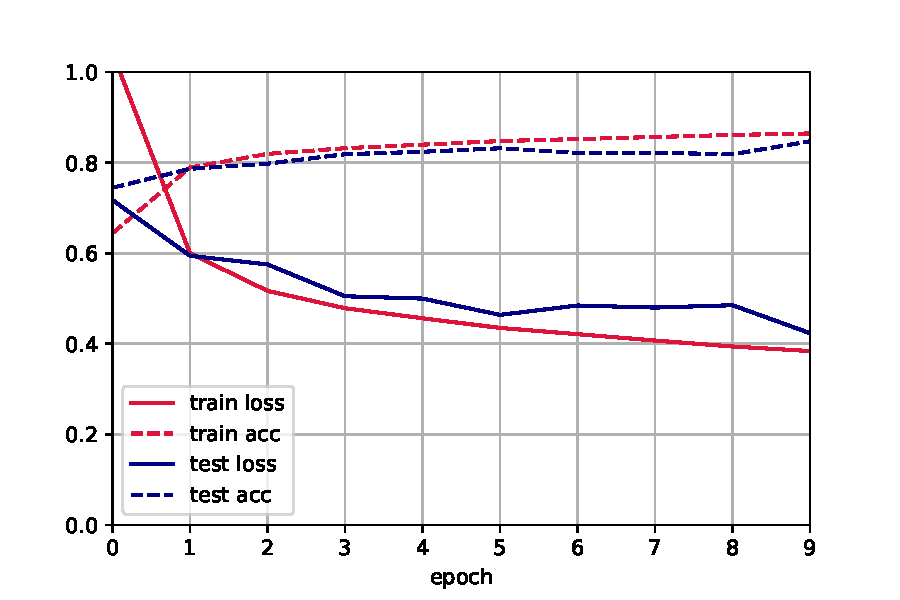
\includegraphics[width=\linewidth]{final_plot}

Code:

\begin{python}
n_inputs = 28 * 28
n_hiddens = 256
n_outputs = 10

W1 = torch.nn.Parameter(0.01 * torch.randn(size=(n_inputs, n_hiddens)))
b1 = torch.nn.Parameter(torch.zeros(size=(1, n_hiddens)))
W2 = torch.nn.Parameter(0.01 * torch.randn(size=(n_hiddens, n_outputs)))
b2 = torch.nn.Parameter(torch.zeros(size=(1, n_outputs)))



def relu(x):
	return x.clamp(min=0)



def softmax(x):
	exped = X.exp()
	return exped / exped.sum(1).reshape(-1, 1)



def net(X):
	X = X.flatten(start_dim=1)
	H = relu(X @ W1 + b1)
	O = softmax(H @ W2 + b2)
	return O



def cross_entropy(y_hat, y):
	y_hat_sub_y = y_hat.gather(1, y.unsqueeze(1)).squeeze()
	return -torch.log(y_hat_sub_y)



def sgd(params, lr=0.1):
	with torch.no_grad():
		for param in params:
			param -= lr * param.grad
			param.grad.zero_()



def train(net, params, train_iter, loss_func=cross_entropy, updater=sgd):
	epochs = 10
	for _ in range(epochs):
		for X, y in train_iter:
			y_hat = net(X)
			losses = loss_func(y_hat, y)
			loss = losses.mean()
			loss.backward()
			updater(params)
\end{python}


\newpage
%%%%%%%%%%%%%%%%%%%%%%%%%%%%%%%%%%%%%%%%%%%%%
% Name and Calibration
%%%%%%%%%%%%%%%%%%%%%%%%%%%%%%%%%%%%%%%%%%%%%
\subsection*{Name}

\subsection*{Collaborators and Resources}
Whom did you work with, and did you use any resources beyond cs181-textbook and your notes?

No one. PyTorch documentation.

\subsection*{Calibration}
Approximately how long did this homework take you to complete (in hours)? 

10

\end{document}
